\section{Simulation study}
\label{sim}

We apply the hierarchical model to simulations from a max-autoregressive process. For $i=1,\ldots,R$, choose $\theta_i\in(0,1]$. Let $W_{i,1}\ldots,W_{i,n}$ be independent unit Fr{\'e}chet random variables, and define
\begin{align}
Y_{i,1} &= W_{i,1}/\theta_i \nonumber \\
Y_{i,j} &= \max\{(1-\theta_i)Y_{i,j-1}, W_{i,j}\}~~~~~j=2,\ldots,n \label{max}
\end{align}
then $Y_{i,\cdot}$ is stochastic process having extremal index $\theta_i$. We let $R=10$, $n=1000$, and $\theta_1=\cdots=\theta_R$. This construction is intended to somewhat mimic our situation with the climate model.

A single threshold is chosen based off a quantile of all simulations taken together. That is, if we wish to choose as a threshold the $0.95$ quantile, then $u$ is the solution to
\[ 0.95 = \sum_{i=1}^R\sum_{j=1}^n\ind(Y_{i,j} \leq u) \]
It is certainly possible to select a threshold $u_i$ for each sequence. While this is expected to yield better estimates for $\theta_i$, it is not immediately clear how to apply model (\ref{gpmod}) in the hierarchical setting with different thresholds. What threshold should be used when calculating return levels for the population distribution? Or a new replicate $Y^*$?

Comparisons between models (\ref{ferro}) and (\ref{suveges}) are made using coverage and RMSE.

Results in Figure \ref{figsim}


\begin{figure}[H]
\begin{center}
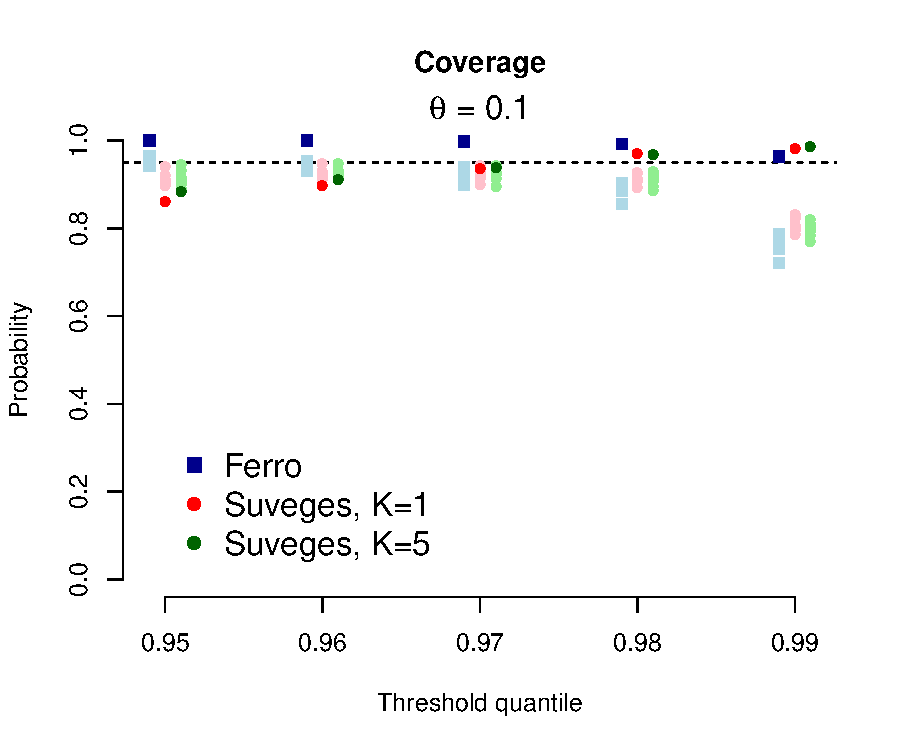
\includegraphics[scale=0.48]{../extremal_comparison/figs/sim_coverage_10.pdf}
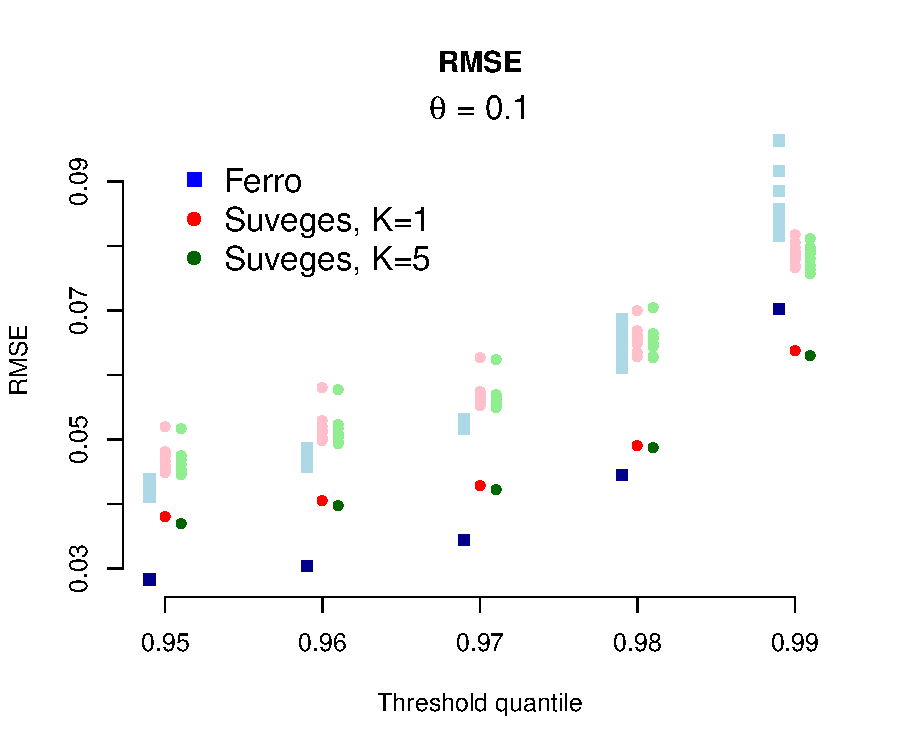
\includegraphics[scale=0.48]{../extremal_comparison/figs/sim_rmse_10.pdf}
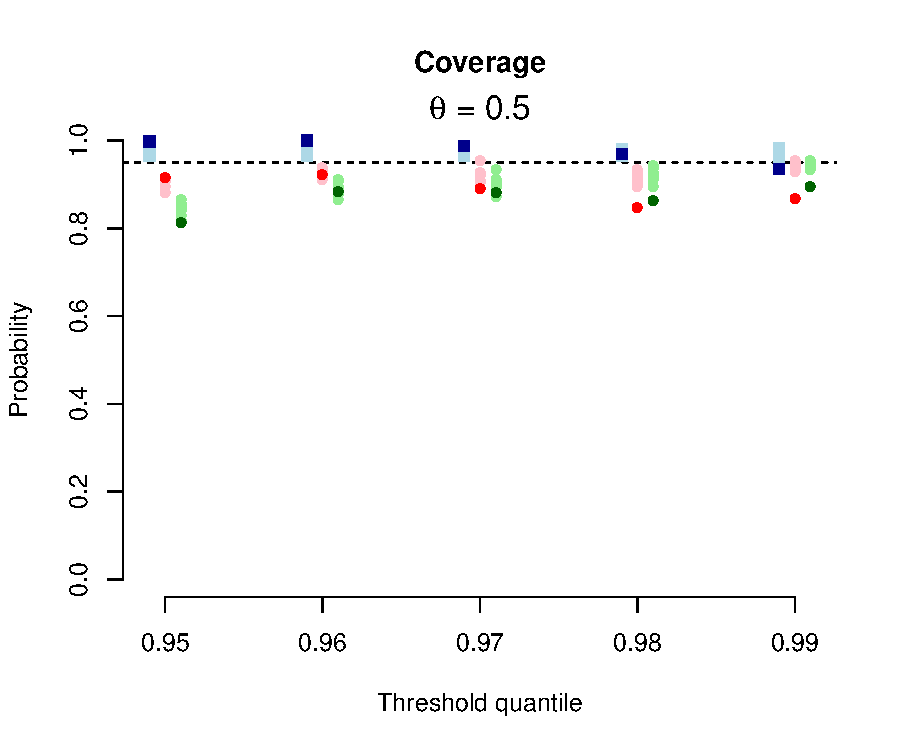
\includegraphics[scale=0.48]{../extremal_comparison/figs/sim_coverage_50.pdf}
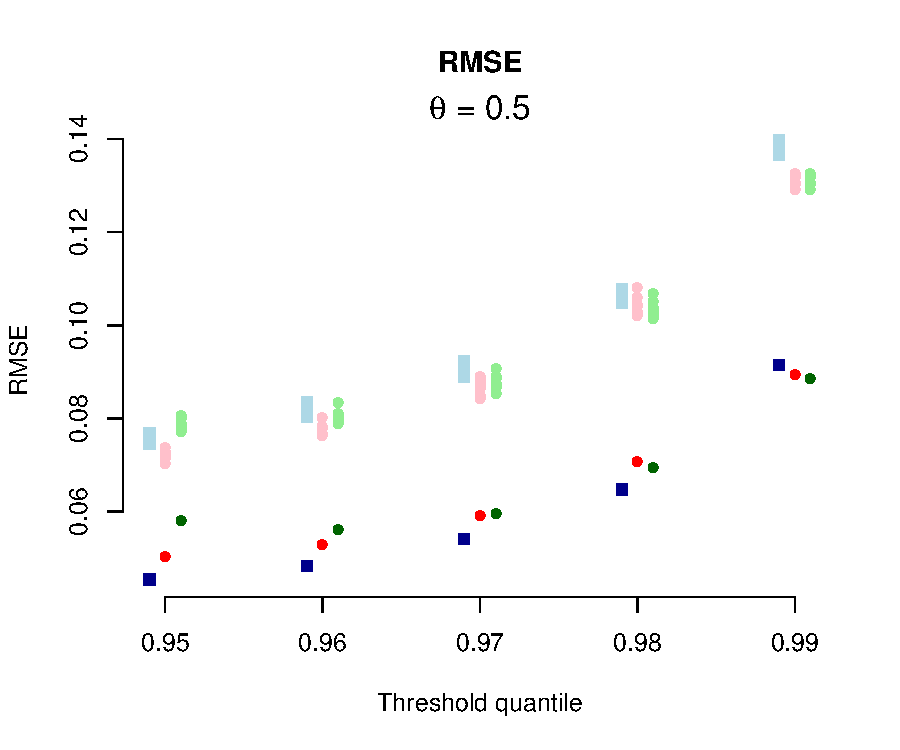
\includegraphics[scale=0.48]{../extremal_comparison/figs/sim_rmse_50.pdf}
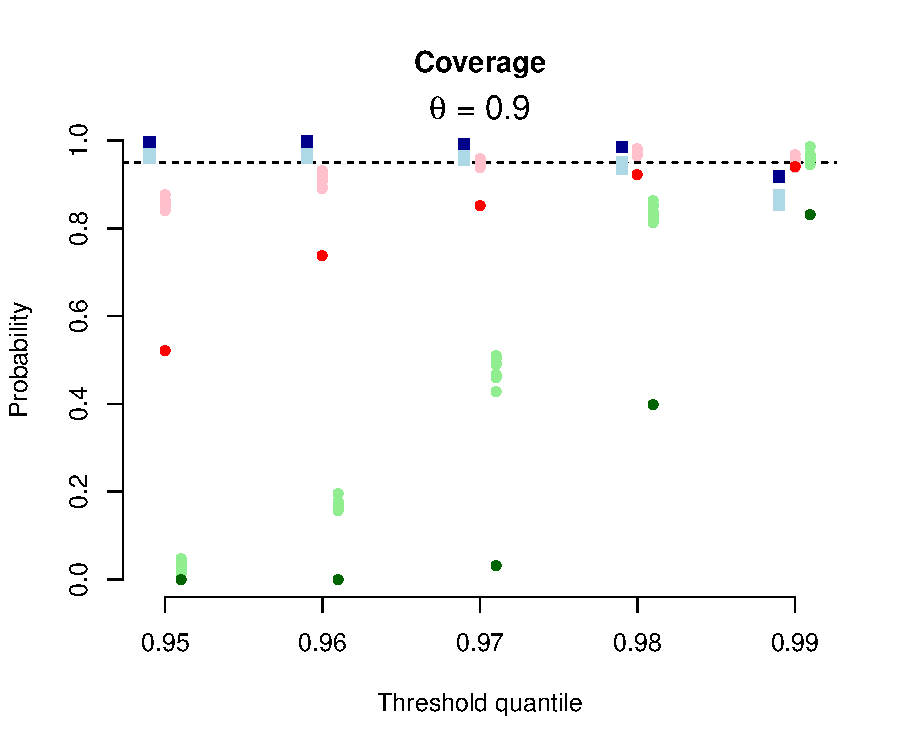
\includegraphics[scale=0.48]{../extremal_comparison/figs/sim_coverage_90.pdf}
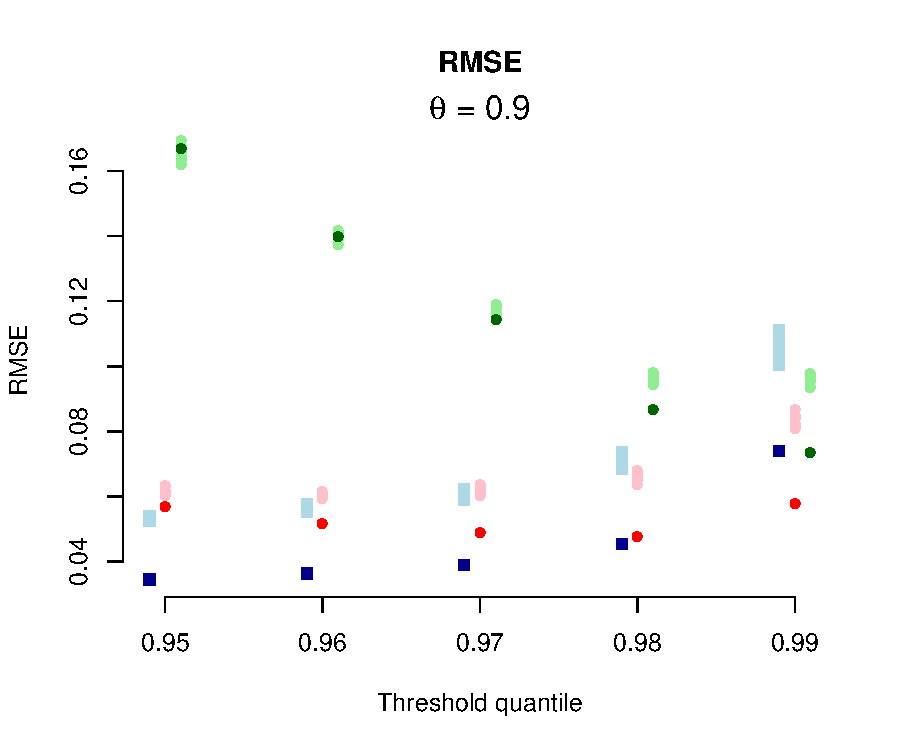
\includegraphics[scale=0.48]{../extremal_comparison/figs/sim_rmse_90.pdf}
\end{center}
\caption{Coverage (left column) and RMSE (right) for the two likelihoods in the simulation study. Each row is based on a different extremal index, either $0.10$, $0.50$, or $0.90$. The darker points represent the hierarchical mean, the lighter points are from the individual sequences. The nominal coverage probability (0.95) is marked by the dashed horizontal line.}
\label{figsim}
\end{figure}
